\documentclass{article}\usepackage[]{graphicx}\usepackage[]{color}
%% maxwidth is the original width if it is less than linewidth
%% otherwise use linewidth (to make sure the graphics do not exceed the margin)
\makeatletter
\def\maxwidth{ %
  \ifdim\Gin@nat@width>\linewidth
    \linewidth
  \else
    \Gin@nat@width
  \fi
}
\makeatother

\definecolor{fgcolor}{rgb}{0.345, 0.345, 0.345}
\newcommand{\hlnum}[1]{\textcolor[rgb]{0.686,0.059,0.569}{#1}}%
\newcommand{\hlstr}[1]{\textcolor[rgb]{0.192,0.494,0.8}{#1}}%
\newcommand{\hlcom}[1]{\textcolor[rgb]{0.678,0.584,0.686}{\textit{#1}}}%
\newcommand{\hlopt}[1]{\textcolor[rgb]{0,0,0}{#1}}%
\newcommand{\hlstd}[1]{\textcolor[rgb]{0.345,0.345,0.345}{#1}}%
\newcommand{\hlkwa}[1]{\textcolor[rgb]{0.161,0.373,0.58}{\textbf{#1}}}%
\newcommand{\hlkwb}[1]{\textcolor[rgb]{0.69,0.353,0.396}{#1}}%
\newcommand{\hlkwc}[1]{\textcolor[rgb]{0.333,0.667,0.333}{#1}}%
\newcommand{\hlkwd}[1]{\textcolor[rgb]{0.737,0.353,0.396}{\textbf{#1}}}%
\let\hlipl\hlkwb

\usepackage{framed}
\makeatletter
\newenvironment{kframe}{%
 \def\at@end@of@kframe{}%
 \ifinner\ifhmode%
  \def\at@end@of@kframe{\end{minipage}}%
  \begin{minipage}{\columnwidth}%
 \fi\fi%
 \def\FrameCommand##1{\hskip\@totalleftmargin \hskip-\fboxsep
 \colorbox{shadecolor}{##1}\hskip-\fboxsep
     % There is no \\@totalrightmargin, so:
     \hskip-\linewidth \hskip-\@totalleftmargin \hskip\columnwidth}%
 \MakeFramed {\advance\hsize-\width
   \@totalleftmargin\z@ \linewidth\hsize
   \@setminipage}}%
 {\par\unskip\endMakeFramed%
 \at@end@of@kframe}
\makeatother

\definecolor{shadecolor}{rgb}{.97, .97, .97}
\definecolor{messagecolor}{rgb}{0, 0, 0}
\definecolor{warningcolor}{rgb}{1, 0, 1}
\definecolor{errorcolor}{rgb}{1, 0, 0}
\newenvironment{knitrout}{}{} % an empty environment to be redefined in TeX

\usepackage{alltt}
\IfFileExists{upquote.sty}{\usepackage{upquote}}{}
\begin{document}

\title{netDx use case: 4-way classification: Medulloblastoma tumour subtype}
\author{Shraddha Pai}
\date{Last updated: 7 September, 2016}

\maketitle

\section{Introduction}
Northcott et al. (2011) identified four subtypes of primary medulloblastoma tumours based on gene expression profiles, each predictable by levels of ~5 genes (Ref 1). For each tumour, we have gene-level expression data (GSE21140) from the Affymetrix Human Exon 1.0 ST array (gene-level). In this application, our goal is to classify a new tumour into one of the 4 subtypes.
\par
The netDx workflow is shown in Figure 1. We use gene signatures identified by previous research and omit the feature selection step. Instead, GeneMANIA (GM) is used to predict tumour labels. For each of the 4 subtypes, we construct a GM database that contains genes part of the corresponding gene signature. Samples from each subtype are split into training (70\%) and test (30\%). One query is run for each of the four subtypes, using the training samples for the corresponding subtypes as a query. In this way, each test sample is ranked by all 4 databases. After test samples have been ranked by all four GeneMANIA queries , each set of ranks is normalized to range between 0 and 1.  The patient is assigned to the class with the highest rank.

\begin{figure}[ht]
\begin{center}
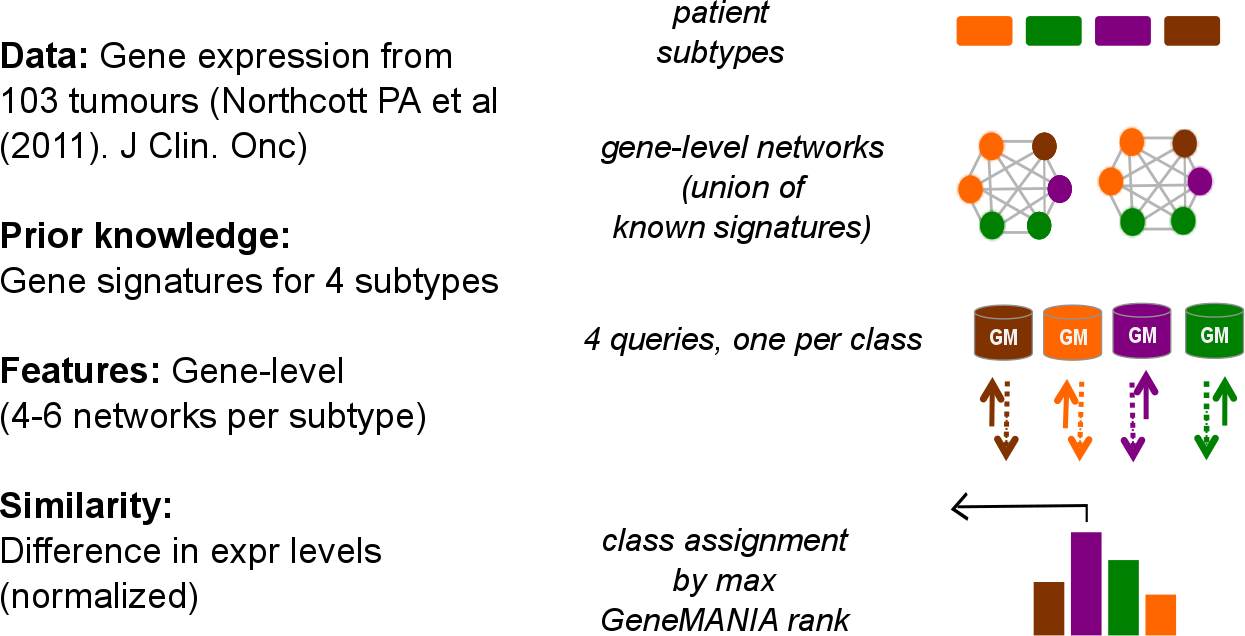
\includegraphics[width=\textwidth]{mblastoma.png}
\caption{netDx workflow for a 4-way classification of medulloblastoma tumour from known gene signatures. \newline A. A GeneMANIA database is built for each subtype. The networks are at the gene-level, with a custom similarity metric (see Section 3); each subtype-specific database contains networks for the genes in the corresponding subtype signature. The networks and database contain all training and test patients. \newline B. A sample is classified by running four GeneMANIA queries, one per subtype. In each case, the query comprises of training samples for that subtype. The query results in subtype-specific similarity ranking. After such ranks have been obtained for all four subtypes, the sample is assigned to the class for which it has the highest rank.}
\end{center}
\end{figure}

\section{Set up}
\subsection{Set up working environment}
\begin{knitrout}
\definecolor{shadecolor}{rgb}{0.969, 0.969, 0.969}\color{fgcolor}\begin{kframe}
\begin{alltt}
\hlstd{outDir} \hlkwb{<-}  \hlkwd{sprintf}\hlstd{(}\hlstr{"%s/MB"}\hlstd{,}\hlkwd{getwd}\hlstd{())}
\hlkwa{if} \hlstd{(}\hlkwd{file.exists}\hlstd{(outDir))} \hlkwd{unlink}\hlstd{(outDir,}\hlkwc{recursive}\hlstd{=}\hlnum{TRUE}\hlstd{)}
\hlkwd{dir.create}\hlstd{(outDir)}

\hlstd{numCores}    \hlkwb{<-} \hlnum{2L}       \hlcom{# number of cores for parallel processing}
\hlstd{pctTrain}    \hlkwb{<-} \hlnum{0.7}      \hlcom{# fraction of samples to use for feature selection}

\hlkwd{require}\hlstd{(netDx)}
\hlkwd{require}\hlstd{(netDx.examples)}
\end{alltt}
\end{kframe}
\end{knitrout}

Load the example data
\begin{knitrout}
\definecolor{shadecolor}{rgb}{0.969, 0.969, 0.969}\color{fgcolor}\begin{kframe}
\begin{alltt}
\hlcom{# Load the Medulloblastoma dataset}
\hlkwd{data}\hlstd{(MBlastoma)}
\end{alltt}
\end{kframe}
\end{knitrout}

\subsection{Define gene signatures}

\begin{knitrout}
\definecolor{shadecolor}{rgb}{0.969, 0.969, 0.969}\color{fgcolor}\begin{kframe}
\begin{alltt}
\hlcom{# subtypes and genes predictive of these. From Table 1 of PMC3306784}
\hlcom{# http://www.ncbi.nlm.nih.gov/pmc/articles/PMC3306784/table/Tab1/}
\hlstd{groupSig} \hlkwb{<-} \hlkwd{list}\hlstd{(}
    \hlkwc{WNT}\hlstd{=}\hlkwd{c}\hlstd{(}\hlstr{"WIF1"}\hlstd{,}\hlstr{"TNC"}\hlstd{,}\hlstr{"GAD"}\hlstd{,}\hlstr{"DKK2"}\hlstd{,}\hlstr{"EMX2"}\hlstd{),}
    \hlkwc{SHH}\hlstd{=}\hlkwd{c}\hlstd{(}\hlstr{"PDLIM3"}\hlstd{,}\hlstr{"EYA1"}\hlstd{,}\hlstr{"HHIP"}\hlstd{,}\hlstr{"ATOH1"}\hlstd{,}\hlstr{"SFRP1"}\hlstd{),}
    \hlkwc{Group3}\hlstd{=}\hlkwd{c}\hlstd{(}\hlstr{"IMPG2"}\hlstd{,}\hlstr{"GABRA5"}\hlstd{,}\hlstr{"EGFL11"}\hlstd{,}\hlstr{"NRL"}\hlstd{,}\hlstr{"MAB21L2"}\hlstd{,}\hlstr{"NPR3"}\hlstd{),}
    \hlkwc{Group4}\hlstd{=}\hlkwd{c}\hlstd{(}\hlstr{"KCNA1"}\hlstd{,}\hlstr{"EOMES"}\hlstd{,}\hlstr{"KHDRBS2"}\hlstd{,}\hlstr{"RBM24"}\hlstd{,}\hlstr{"UNC5D"}\hlstd{,}\hlstr{"OAS1"}\hlstd{)}
\hlstd{)}
\end{alltt}
\end{kframe}
\end{knitrout}

\subsection{Split samples into train and test}

For this example we manually separate samples from each of the 4 subtypes into 70\% training and 30\% test
\begin{knitrout}
\definecolor{shadecolor}{rgb}{0.969, 0.969, 0.969}\color{fgcolor}\begin{kframe}
\begin{alltt}
\hlcom{# ---------------------------------------------}
\hlcom{# split dataset into train/test in group-wise manner. Note that we }
\hlcom{# include patients not in any particular group because they serve}
\hlcom{# as negatives}
\hlkwd{set.seed}\hlstd{(}\hlnum{42}\hlstd{)} \hlcom{# make reproducible}
\hlstd{TT_STATUS} \hlkwb{<-} \hlkwd{character}\hlstd{(}\hlkwd{nrow}\hlstd{(MB.pheno))}
\hlkwa{for} \hlstd{(g} \hlkwa{in} \hlkwd{unique}\hlstd{(MB.pheno}\hlopt{$}\hlstd{STATUS)) \{}
    \hlstd{idx} \hlkwb{<-} \hlkwd{which}\hlstd{(MB.pheno}\hlopt{$}\hlstd{STATUS} \hlopt \hlstd{g)}
    \hlstd{status} \hlkwb{<-} \hlkwd{rep}\hlstd{(}\hlstr{"TEST"}\hlstd{,}\hlkwd{length}\hlstd{(idx))}
    \hlstd{status[}\hlnum{1}\hlopt{:}\hlstd{(}\hlkwd{floor}\hlstd{(pctTrain} \hlopt{*} \hlkwd{length}\hlstd{(idx)))]} \hlkwb{<-} \hlstr{"TRAIN"}
    \hlstd{TT_STATUS[idx]} \hlkwb{<-} \hlkwd{sample}\hlstd{(status,} \hlkwc{replace}\hlstd{=}\hlnum{FALSE}\hlstd{)} \hlcom{# scramble}
\hlstd{\}}
\hlstd{MB.pheno} \hlkwb{<-} \hlkwd{cbind}\hlstd{(MB.pheno,} \hlkwc{TT_STATUS}\hlstd{=TT_STATUS)}
\end{alltt}
\end{kframe}
\end{knitrout}

\section{Build predictor for each subtype}
In this example, we skip feature selection and move straight to predicting subtypes for test tumours, based on similarity to training samples.

\begin{knitrout}
\definecolor{shadecolor}{rgb}{0.969, 0.969, 0.969}\color{fgcolor}\begin{kframe}
\begin{alltt}
\hlstd{MB.pheno_train} \hlkwb{<-} \hlkwd{subset}\hlstd{(MB.pheno, TT_STATUS} \hlopt \hlstr{"TRAIN"}\hlstd{)}
\end{alltt}
\end{kframe}
\end{knitrout}

For each subtype, we build a GeneMANIA database consisting of features for that subtype.  Each database contains all 103 samples. Features are at the levels of genes. The similarity measure is a custom-defined one, here seen in the \texttt{geneSim()} function.

\begin{knitrout}
\definecolor{shadecolor}{rgb}{0.969, 0.969, 0.969}\color{fgcolor}\begin{kframe}
\begin{alltt}
\hlcom{# custom similarity measure}
\hlstd{geneSim} \hlkwb{<-} \hlkwa{function}\hlstd{(}\hlkwc{x}\hlstd{) \{}
    \hlkwa{if} \hlstd{(}\hlkwd{nrow}\hlstd{(x)}\hlopt{>=}\hlnum{1}\hlstd{) x} \hlkwb{<-} \hlstd{x[}\hlnum{1}\hlstd{,]}
    \hlstd{nm} \hlkwb{<-} \hlkwd{colnames}\hlstd{(x)}
    \hlstd{x} \hlkwb{<-} \hlkwd{as.numeric}\hlstd{(x)}
    \hlstd{n} \hlkwb{<-} \hlkwd{length}\hlstd{(x)}
    \hlstd{rngX}  \hlkwb{<-} \hlkwd{max}\hlstd{(x)}\hlopt{-}\hlkwd{min}\hlstd{(x)}

    \hlstd{out} \hlkwb{<-} \hlkwd{matrix}\hlstd{(}\hlnum{NA}\hlstd{,}\hlkwc{nrow}\hlstd{=n,}\hlkwc{ncol}\hlstd{=n);}
    \hlcom{# weight between i and j is}
    \hlcom{# wt(i,j) = 1 - (abs(g[i]-g[j])/(max(g)-min(g)))}
    \hlcom{# where g is the eMB.xpression vector for each gene}
    \hlkwa{for} \hlstd{(j} \hlkwa{in} \hlnum{1}\hlopt{:}\hlstd{n) out[,j]} \hlkwb{<-} \hlnum{1}\hlopt{-}\hlstd{(}\hlkwd{abs}\hlstd{((x}\hlopt{-}\hlstd{x[j])}\hlopt{/}\hlstd{rngX))}
    \hlkwd{rownames}\hlstd{(out)} \hlkwb{<-} \hlstd{nm;} \hlkwd{colnames}\hlstd{(out)}\hlkwb{<-} \hlstd{nm}
    \hlstd{out}
\hlstd{\}}
\end{alltt}
\end{kframe}
\end{knitrout}

For each subtype, the loop combines the following steps:
\begin{itemize}
\item \texttt{makePSN\_NamedMatrix()}: Function that creates the patient networks from the expression vector. Here we supply the custom similarity-computing function via the \texttt{customFunc} argument. The interaction networks are written in the directory \texttt{netDir}.
\item \texttt{GM\_createDB()}: All the input networks in \texttt{netDir} are integrated into a single GeneMANIA database.
\item \texttt{GM\_writeQueryFile()}: Write a GeneMANIA query file; the GeneMANIA query will obtain a similarity ranking for test patients
\item \texttt{runGeneMANIA()}: Runs a GeneMANIA query
\item \texttt{GM\_getQueryROC()}: Process the patient ranking output file (the \texttt{.prank} file)
\end{itemize}

\begin{knitrout}
\definecolor{shadecolor}{rgb}{0.969, 0.969, 0.969}\color{fgcolor}\begin{kframe}
\begin{alltt}
\hlcom{# directories with group-specific predictors}
\hlstd{predRes} \hlkwb{<-} \hlkwd{list}\hlstd{()}
\hlcom{## for each subtype}
\hlkwa{for} \hlstd{(g} \hlkwa{in} \hlkwd{names}\hlstd{(groupSig))\{}
    \hlstd{pDir} \hlkwb{<-} \hlkwd{sprintf}\hlstd{(}\hlstr{"%s/%s"}\hlstd{,outDir,g)}
    \hlkwd{dir.create}\hlstd{(pDir)}

    \hlcom{# each gene has its own PSN}
    \hlstd{sigNets} \hlkwb{<-} \hlkwd{list}\hlstd{()}
    \hlkwa{for} \hlstd{(g2} \hlkwa{in} \hlstd{groupSig[[g]]) sigNets[[g2]]} \hlkwb{<-} \hlstd{g2}

    \hlcom{# create patient networks using train & test samples}
    \hlcom{# networks are limited to signature genes for this subtype}
    \hlstd{idx}     \hlkwb{<-} \hlkwd{which}\hlstd{(MB.xpr_names} \hlopt \hlstd{groupSig[[g]])}
    \hlkwd{cat}\hlstd{(}\hlkwd{sprintf}\hlstd{(}\hlstr{"Subtype : %s \{ %s \} => %i measures\textbackslash{}n"}\hlstd{,}
                \hlstd{g,} \hlkwd{paste}\hlstd{(groupSig[[g]],}\hlkwc{collapse}\hlstd{=}\hlstr{","}\hlstd{),} \hlkwd{length}\hlstd{(idx)))}
    \hlstd{netDir}  \hlkwb{<-} \hlkwd{sprintf}\hlstd{(}\hlstr{"%s/networks"}\hlstd{,pDir)}

    \hlcom{# this function call creates the PSN}
    \hlstd{netList} \hlkwb{<-} \hlkwd{makePSN_NamedMatrix}\hlstd{(MB.xpr[idx,], MB.xpr_names[idx],}
                                   \hlstd{sigNets,netDir,}
                                   \hlkwc{simMetric}\hlstd{=}\hlstr{"custom"}\hlstd{,}\hlkwc{customFunc}\hlstd{=geneSim,}
                                   \hlkwc{verbose}\hlstd{=}\hlnum{TRUE}\hlstd{)}

    \hlcom{# create a GeneMANIA database out of these networks}
    \hlstd{dbDir} \hlkwb{<-} \hlkwd{GM_createDB}\hlstd{(netDir, MB.pheno}\hlopt{$}\hlstd{ID, pDir)}

    \hlcom{# run a query using training samples for this subtype.}
    \hlcom{# get ranking for all patients in the database by running GeneMANIA}
    \hlstd{trainSamps} \hlkwb{<-} \hlstd{MB.pheno}\hlopt{$}\hlstd{ID[}\hlkwd{which}\hlstd{(MB.pheno}\hlopt{$}\hlstd{TT_STATUS} \hlopt \hlstr{"TRAIN"}
                \hlopt{&} \hlstd{MB.pheno}\hlopt{$}\hlstd{STATUS} \hlopt \hlstd{g)]}
    \hlstd{qFile}      \hlkwb{<-} \hlkwd{sprintf}\hlstd{(}\hlstr{"%s/query.txt"}\hlstd{, pDir)}
    \hlkwd{GM_writeQueryFile}\hlstd{(trainSamps,} \hlstr{"all"}\hlstd{,} \hlkwd{nrow}\hlstd{(MB.pheno),qFile)}
    \hlstd{resFile} \hlkwb{<-} \hlkwd{runGeneMANIA}\hlstd{(dbDir}\hlopt{$}\hlstd{dbDir, qFile, pDir)}

    \hlcom{# compute ROC curve for each predictor}
    \hlstd{predRes[[g]]} \hlkwb{<-} \hlkwd{GM_getQueryROC}\hlstd{(}\hlkwd{sprintf}\hlstd{(}\hlstr{"%s.PRANK"}\hlstd{,resFile),}
            \hlstd{MB.pheno, g)}
\hlstd{\}}
\end{alltt}
\begin{verbatim}
## Subtype : WNT { WIF1,TNC,GAD,DKK2,EMX2 } => 4 measures
## Got 4 networks
## 	* Creating placeholder files
## 	* Populating database files, recoding identifiers
## 	* Build GeneMANIA index
## 	* Build GeneMANIA cache
## 	 * Cleanup[1] "java -d64 -Xmx6G -cp /Library/Frameworks/R.framework/Versions/3.3/Resources/library/netDx/java/GeneMANIA-3.2B7.jar org.genemania.plugin.apps.QueryRunner  --data /Users/ahmadshah/netDx_fork/examples/MB/WNT/dataset --in flat --out flat --threads 1 --results /Users/ahmadshah/netDx_fork/examples/MB/WNT /Users/ahmadshah/netDx_fork/examples/MB/WNT/query.txt 2>&1 > /Users/ahmadshah/netDx_fork/examples/MB/WNT/query.txt.log"
## * Attempt 1 : query.txt
## QueryRunner time taken: 7.9 s
## Subtype : SHH { PDLIM3,EYA1,HHIP,ATOH1,SFRP1 } => 5 measures
## Got 5 networks
## 	* Creating placeholder files
## 	* Populating database files, recoding identifiers
## 	* Build GeneMANIA index
## 	* Build GeneMANIA cache
## 	 * Cleanup[1] "java -d64 -Xmx6G -cp /Library/Frameworks/R.framework/Versions/3.3/Resources/library/netDx/java/GeneMANIA-3.2B7.jar org.genemania.plugin.apps.QueryRunner  --data /Users/ahmadshah/netDx_fork/examples/MB/SHH/dataset --in flat --out flat --threads 1 --results /Users/ahmadshah/netDx_fork/examples/MB/SHH /Users/ahmadshah/netDx_fork/examples/MB/SHH/query.txt 2>&1 > /Users/ahmadshah/netDx_fork/examples/MB/SHH/query.txt.log"
## * Attempt 1 : query.txt
## QueryRunner time taken: 8.2 s
## Subtype : Group3 { IMPG2,GABRA5,EGFL11,NRL,MAB21L2,NPR3 } => 6 measures
## Got 5 networks
## 	* Creating placeholder files
## 	* Populating database files, recoding identifiers
## 	* Build GeneMANIA index
## 	* Build GeneMANIA cache
## 	 * Cleanup[1] "java -d64 -Xmx6G -cp /Library/Frameworks/R.framework/Versions/3.3/Resources/library/netDx/java/GeneMANIA-3.2B7.jar org.genemania.plugin.apps.QueryRunner  --data /Users/ahmadshah/netDx_fork/examples/MB/Group3/dataset --in flat --out flat --threads 1 --results /Users/ahmadshah/netDx_fork/examples/MB/Group3 /Users/ahmadshah/netDx_fork/examples/MB/Group3/query.txt 2>&1 > /Users/ahmadshah/netDx_fork/examples/MB/Group3/query.txt.log"
## * Attempt 1 : query.txt
## QueryRunner time taken: 8.3 s
## Subtype : Group4 { KCNA1,EOMES,KHDRBS2,RBM24,UNC5D,OAS1 } => 6 measures
## Got 6 networks
## 	* Creating placeholder files
## 	* Populating database files, recoding identifiers
## 	* Build GeneMANIA index
## 	* Build GeneMANIA cache
## 	 * Cleanup[1] "java -d64 -Xmx6G -cp /Library/Frameworks/R.framework/Versions/3.3/Resources/library/netDx/java/GeneMANIA-3.2B7.jar org.genemania.plugin.apps.QueryRunner  --data /Users/ahmadshah/netDx_fork/examples/MB/Group4/dataset --in flat --out flat --threads 1 --results /Users/ahmadshah/netDx_fork/examples/MB/Group4 /Users/ahmadshah/netDx_fork/examples/MB/Group4/query.txt 2>&1 > /Users/ahmadshah/netDx_fork/examples/MB/Group4/query.txt.log"
## * Attempt 1 : query.txt
## QueryRunner time taken: 8.6 s
\end{verbatim}
\end{kframe}
\end{knitrout}

\section{Evaluate performance}
Once we have run GeneMANIA on all 4 subclasses, the patient gets assigned to the class for which it has the highest ranking.

Take a look at the ROC curves.
\begin{knitrout}
\definecolor{shadecolor}{rgb}{0.969, 0.969, 0.969}\color{fgcolor}\begin{kframe}
\begin{alltt}
\hlkwd{par}\hlstd{(}\hlkwc{mfrow}\hlstd{=}\hlkwd{c}\hlstd{(}\hlnum{2}\hlstd{,}\hlnum{2}\hlstd{))}
\hlstd{tmp} \hlkwb{<-} \hlkwd{sapply}\hlstd{(}\hlkwd{names}\hlstd{(predRes),} \hlkwa{function}\hlstd{(}\hlkwc{nm}\hlstd{)\{}
    \hlstd{x} \hlkwb{<-} \hlstd{predRes[[nm]]}
    \hlkwd{plot}\hlstd{(x}\hlopt{$}\hlstd{roc,}
         \hlkwc{main}\hlstd{=}\hlkwd{sprintf}\hlstd{(}\hlstr{"%s: N=%i (AUC=%1.3f)"}\hlstd{,}
                      \hlstd{nm,}\hlkwd{length}\hlstd{(x}\hlopt{$}\hlstd{roc}\hlopt{@}\hlkwc{x.values}\hlstd{[[}\hlnum{1}\hlstd{]]),x}\hlopt{$}\hlstd{auc),}
         \hlkwc{cex.main}\hlstd{=}\hlnum{0.8}\hlstd{)}
    \hlstd{\})}
\end{alltt}
\end{kframe}
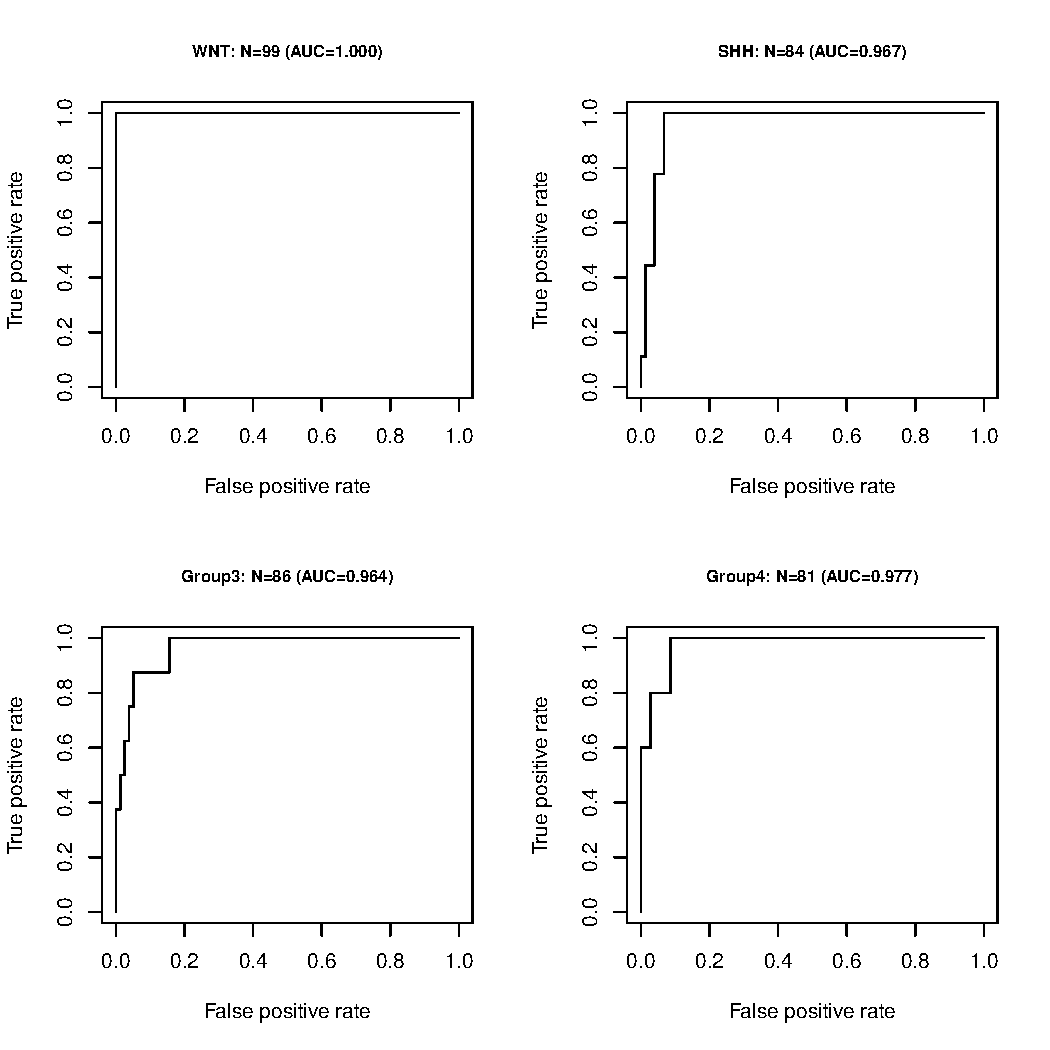
\includegraphics[width=\maxwidth]{figure/unnamed-chunk-8-1} 
\begin{kframe}\begin{alltt}
\hlkwd{save}\hlstd{(predRes,}\hlkwc{file}\hlstd{=}\hlkwd{sprintf}\hlstd{(}\hlstr{"%s/predictions.Rdata"}\hlstd{,outDir))}
\end{alltt}
\end{kframe}
\end{knitrout}


Finally, predict the class of each test sample
\begin{knitrout}
\definecolor{shadecolor}{rgb}{0.969, 0.969, 0.969}\color{fgcolor}\begin{kframe}
\begin{alltt}
\hlstd{predClass}       \hlkwb{<-} \hlkwd{GM_OneVAll_getClass}\hlstd{(predRes)}
\end{alltt}
\begin{verbatim}
## *** 66 rows have an NA prediction (probably query samples that were not not ranked
\end{verbatim}
\begin{alltt}
\hlstd{testSamps}       \hlkwb{<-} \hlkwd{merge}\hlstd{(}\hlkwc{x}\hlstd{=MB.pheno,}\hlkwc{y}\hlstd{=predClass,}\hlkwc{by}\hlstd{=}\hlstr{"ID"}\hlstd{)}
\hlstd{testSamps}       \hlkwb{<-} \hlstd{testSamps[}\hlopt{-}\hlkwd{which}\hlstd{(}\hlopt{!}\hlstd{testSamps}\hlopt{$}\hlstd{STATUS} \hlopt \hlkwd{c}\hlstd{(}\hlstr{"WNT"}\hlstd{,}\hlstr{"SHH"}\hlstd{,}
                                \hlstr{"Group3"}\hlstd{,}\hlstr{"Group4"}\hlstd{)),]}
\end{alltt}
\end{kframe}
\end{knitrout}

Compute class match accuracy
\begin{knitrout}
\definecolor{shadecolor}{rgb}{0.969, 0.969, 0.969}\color{fgcolor}\begin{kframe}
\begin{alltt}
\hlstd{rightClass} \hlkwb{<-} \hlstd{testSamps}\hlopt{$}\hlstd{STATUS} \hlopt{==} \hlstd{testSamps}\hlopt{$}\hlstd{PRED_CLASS}
\hlstd{numCor} \hlkwb{<-} \hlkwd{sum}\hlstd{(rightClass); ln} \hlkwb{<-} \hlkwd{nrow}\hlstd{(testSamps)}
\hlkwd{cat}\hlstd{(}\hlkwd{sprintf}\hlstd{(}\hlstr{"Overall classifier accuracy = %i of %i  (%i%%)"}\hlstd{,}
            \hlstd{numCor, ln,} \hlkwd{round}\hlstd{((numCor}\hlopt{/}\hlstd{ln)}\hlopt{*}\hlnum{100}\hlstd{)))}
\end{alltt}
\begin{verbatim}
## Overall classifier accuracy = 28 of 30  (93%)
\end{verbatim}
\end{kframe}
\end{knitrout}

Examine class-specific accuracy:
\begin{knitrout}
\definecolor{shadecolor}{rgb}{0.969, 0.969, 0.969}\color{fgcolor}\begin{kframe}
\begin{alltt}
\hlkwa{for} \hlstd{(g} \hlkwa{in} \hlkwd{names}\hlstd{(groupSig))\{}
    \hlstd{idx} \hlkwb{<-} \hlkwd{which}\hlstd{(testSamps}\hlopt{$}\hlstd{STATUS} \hlopt \hlstd{g)}
    \hlstd{numCor} \hlkwb{<-} \hlkwd{sum}\hlstd{(rightClass[idx]); ln} \hlkwb{<-} \hlkwd{length}\hlstd{(idx)}
    \hlkwd{cat}\hlstd{(}\hlkwd{sprintf}\hlstd{(}\hlstr{"\textbackslash{}t%s = %i of %i  (%i%%)\textbackslash{}n"}\hlstd{,}
            \hlstd{g, numCor, ln,} \hlkwd{round}\hlstd{((numCor}\hlopt{/}\hlstd{ln)}\hlopt{*}\hlnum{100}\hlstd{)))}
\hlstd{\}}
\end{alltt}
\begin{verbatim}
## 	WNT = 3 of 3  (100%)
## 	SHH = 9 of 9  (100%)
## 	Group3 = 7 of 8  (88%)
## 	Group4 = 9 of 10  (90%)
\end{verbatim}
\end{kframe}
\end{knitrout}

\section{sessionInfo}
\begin{knitrout}
\definecolor{shadecolor}{rgb}{0.969, 0.969, 0.969}\color{fgcolor}\begin{kframe}
\begin{alltt}
\hlkwd{sessionInfo}\hlstd{()}
\end{alltt}
\begin{verbatim}
## R version 3.3.3 (2017-03-06)
## Platform: x86_64-apple-darwin13.4.0 (64-bit)
## Running under: macOS Sierra 10.12.5
## 
## locale:
## [1] en_CA.UTF-8/en_CA.UTF-8/en_CA.UTF-8/C/en_CA.UTF-8/en_CA.UTF-8
## 
## attached base packages:
## [1] stats4    parallel  stats     graphics  grDevices utils     datasets 
## [8] methods   base     
## 
## other attached packages:
##  [1] netDx.examples_0.0.0.9000 netDx_0.9242             
##  [3] RColorBrewer_1.1-2        pracma_2.0.7             
##  [5] ROCR_1.0-7                gplots_3.0.1             
##  [7] GenomicRanges_1.26.4      GenomeInfoDb_1.10.3      
##  [9] IRanges_2.8.2             S4Vectors_0.12.2         
## [11] BiocGenerics_0.20.0       combinat_0.0-8           
## [13] doParallel_1.0.10         iterators_1.0.8          
## [15] foreach_1.4.3             bigmemory_4.5.19         
## [17] bigmemory.sri_0.1.3       knitr_1.16               
## 
## loaded via a namespace (and not attached):
##  [1] igraph_1.0.1       Rcpp_0.12.11       XVector_0.14.1    
##  [4] magrittr_1.5       zlibbioc_1.20.0    quadprog_1.5-5    
##  [7] highr_0.6          plyr_1.8.4         stringr_1.2.0     
## [10] caTools_1.17.1     tools_3.3.3        KernSmooth_2.23-15
## [13] gtools_3.5.0       reshape2_1.4.2     bitops_1.0-6      
## [16] codetools_0.2-15   RCurl_1.95-4.8     evaluate_0.10     
## [19] gdata_2.18.0       stringi_1.1.5      compiler_3.3.3
\end{verbatim}
\end{kframe}
\end{knitrout}

\section{References}
1. Northcott PA et al. (2011). J Clin Oncol. 29 (11):1408.
\end{document}
